% interactapasample.tex
% v1.05 - August 2017

\documentclass[]{interact}

\usepackage[caption=false]{subfig}% Support for small, `sub' figures and tables
%\usepackage[nolists,tablesfirst]{endfloat}% To `separate' figures and tables from text if required
% \usepackage[doublespacing]{setspace}% To produce a `double spaced' document if required
% \setlength\parindent{24pt}% To increase paragraph indentation when line spacing is doubled

\usepackage[ruled,linesnumbered]{algorithm2e}
\newcommand{\balg}[1][htbp]{\begin{algorithm}[#1]\DontPrintSemicolon}
\newcommand{\ealg}{\end{algorithm}}

\usepackage{interval}
\intervalconfig{soft open fences}

\usepackage{pgf}
\pgfdeclarelayer{background}
\pgfsetlayers{background,main}

\usepackage{standalone}
\usepackage{subfig}
\usepackage{tikz}
\usetikzlibrary{%
    arrows,
    arrows.meta,
    backgrounds,
    decorations.pathreplacing,
    decorations.text,
    patterns,
    positioning,
    shapes.arrows,
    shapes.geometric
}


\tikzstyle{every picture} += [remember picture]
\tikzstyle{na} = [baseline=-.5ex]

\tikzset{%
    queue/.pic={%
        code{%
            \node (rect) at (38.5mm, 10mm) {};
            \draw[thick] (0, 0) -- ++(40mm, 0) -- ++(0, 20mm) -- ++(-40mm, 0);
            \foreach \val in {0, ..., #1}{%
                \draw[thick] ([xshift=-\val*5mm] 40mm, 20mm) -- ++(0, -20mm);
            };

            \foreach \val/\lab/\size in {%
                0/1/\scriptsize,
                1/2/\scriptsize,
                3/c-1/\tiny,
                4/c/\scriptsize%
            }{%
                \node[draw, circle, thick, minimum size=9.5mm] (\lab)
                    at (55mm, 29mm - \val * 9.5mm) {\size$\lab$};
                \draw[-latex, thick] (rect.east) -- (\lab.west);
            };

            \node at (55mm, 11mm) {$\vdots$};
            \node at (5mm, 10mm) {$\cdots$};
        };
    },
    myarrow/.style={%
        line width=2mm,
        draw=gray!50,
        -triangle 60,
        postaction={draw=gray!50, line width=4mm, shorten >=6mm, -},
    },
    double -latex/.style args={#1 colored by #2 and #3}{%
        -latex,
        line width=#1,
        #2,
        postaction={%
            draw,
            -latex,
            #3,
            line width=(#1)/3,
            shorten <=(#1)/4,
            shorten >=4.5*(#1)/3
        },
    },
    mypointer/.style={%
        double -latex=1mm colored by gray!50 and gray!50,
    }
}

\newlength{\imgwidth}
\setlength{\imgwidth}{.95\textwidth}
\newlength{\tabwidth}
\setlength{\tabwidth}{.9\textwidth}

\usepackage[natbibapa,nodoi]{apacite}
\setlength\bibhang{12pt}
\renewcommand\bibliographytypesize{\fontsize{10}{12}\selectfont}

\theoremstyle{plain}% Theorem-like structures provided by amsthm.sty
\newtheorem{theorem}{Theorem}[section]
\newtheorem{lemma}[theorem]{Lemma}
\newtheorem{corollary}[theorem]{Corollary}
\newtheorem{proposition}[theorem]{Proposition}

\theoremstyle{definition}
\newtheorem{definition}[theorem]{Definition}
\newtheorem{example}[theorem]{Example}

\theoremstyle{remark}
\newtheorem{remark}{Remark}
\newtheorem{notation}{Notation}

\newcommand{\ctmuhb}{Cwm Taf Morgannwg University Health Board}

\definecolor{blue}{HTML}{0072B2}
\definecolor{green}{HTML}{009E73}
\definecolor{orange}{HTML}{D55E00}
\definecolor{pink}{HTML}{CC79A7}

\DeclareMathOperator*{\argmin}{arg\,min}

%%%%%%%%%%%%%%%%%%%%%%%%%%%%%%%%%%%%%%%%%%%%%%%%%%%%%%%%%%%%%%%%%%%%%%%%%%%%%%%%

\begin{document}

% \articletype{ARTICLE TEMPLATE}% Specify the article type or omit as appropriate

\title{%
  Segmentation analysis and the recovery of queuing parameters via the
  Wasserstein distance: a study of administrative data for patients with chronic
  obstructive pulmonary disease
}

\author{%
  \name{%
    Henry Wilde\textsuperscript{a}%
    \thanks{CONTACT Henry Wilde. Email: henrydavidwilde@gmail.com},
    Vincent Knight\textsuperscript{a},
    Jonathan Gillard\textsuperscript{a}
    and Kendal Smith\textsuperscript{b}
  }
  \affil{%
    \textsuperscript{a}School of Mathematics, Cardiff University, UK;
    \textsuperscript{b}Cwm Taf Morgannwg University Health Board, UK
  }
}

\maketitle

\begin{abstract}
This work uses a data-driven approach to analyse how the resource requirements
of patients with chronic obstructive pulmonary disease (COPD) may change,
quantifying how those changes impact the hospital system with which the patients
interact. This approach is composed of a novel combination of often distinct
modes of analysis: segmentation, operational queuing theory, and the recovery of
parameters from incomplete data. By combining these methods as presented here,
this work demonstrates that potential limitations around the availability of
fine-grained data can be overcome. Thus, finding useful operational results
despite using only administrative data.

The paper begins by finding a useful clustering of the population from this
granular data that feeds into a multi-class \(M/M/c\) model, whose parameters
are recovered from the data via parameterisation and the Wasserstein distance.
This model is then used to conduct an informative analysis of the underlying
queuing system and the needs of the population under study through several
what-if scenarios.

The analyses used to form and study this model consider, in effect, all types of
patient arrivals and how those types impact the system. With that, this study
finds that there are no quick solutions to reduce the impact of COPD patients on
the system, including adding capacity to the system. In this analysis, the only
effective intervention to reduce the strain caused by those presenting with COPD
is to enact external policies which directly improve the overall health of the
COPD population before they arrive at the hospital.
\end{abstract}

\begin{keywords}
OR in health services; machine learning; queuing
\end{keywords}


\section{Introduction}\label{sec:intro}

Population health research is increasingly based on data-driven methods for
patient-centred care --- as opposed to those designed solely by clinical
experts. This movement is borne from the advent of accessible software and a
relative abundance of electronic data. However, many such methods rely heavily
on detailed data about both the healthcare system and its population, which may
limit research where sophisticated data pipelines are not yet in place.

The only healthcare datasets used in this work are administrative hospital
records. These records offer little detail as to the exact nature of a patient's
time in hospital other than a surface-level summary. Exploratory analysis of a
population-wide administrative dataset, omitted from this manuscript, revealed
the presence of high variation in almost all regards. This variability stifles
the possibility of uncovering valuable insights about the whole population.
However, some benefits are made apparent by considering a condition-specific
population. This work utilises another administrative dataset of patients
presenting COPD, and demonstrates how actionable insights can be identified by
thoroughly extracting information from the dataset through the use of machine
learning and operational research techniques.

This manuscript presents a method of overcoming this, using routinely gathered,
administrative hospital data to build a clustering which feeds into a
multi-class queuing model, allowing for better understanding of the healthcare
population and the system with which they interact. COPD is a condition of
particular interest to population health research, and to \ctmuhb, as it is
known to often present as a comorbidity in patients~\citep{Houben2019},
increasing the complexity of treatments among those with the condition.
Moreover, an internal report by NHS Wales found \ctmuhb\ had the highest
prevalence of the condition across all the Welsh health boards.

This work draws upon several overlapping sources within mathematical research,
and this work contributes to the literature in three ways: to theoretical
queuing research by the estimation of missing queuing parameters with the
Wasserstein distance; to operational healthcare research through the weaving
together of the combination of methods used in this work despite data
constraints; and to public health research by adding to the growing body of
mathematical and operational work around a condition that is vital to understand
operationally, socially and medically.

The remainder of this manuscript is structured as follows:

\begin{itemize}
    \item Section~\ref{sec:intro} introduces the paper and provides a literature
        review, followed by an overview of the case study dataset and its
        clustering;
    \item Section~\ref{sec:model} describes the queuing model and the estimation
        of its parameters;
    \item Section~\ref{sec:scenarios} presents several what-if scenarios with
        insight provided by the model parameterisation and the clustering;
    \item Section~\ref{sec:summary} summarises the manuscript and its findings.
\end{itemize}


\subsection{Literature review}\label{subsec:review}

Given the subject matter of this work, the relevant literature spans much of
operational research in healthcare, and the focus of this review is on the
critical topics of segmentation analysis, queuing models applied to hospital
systems, and the handling of missing or incomplete data for such queues.

\subsubsection{Segmentation analysis}

Segmentation analysis allows for the targeted analysis of otherwise
heterogeneous datasets and encompasses several techniques from operational
research, statistics and machine learning. One of the most desirable qualities
of this kind of analysis is the ability to glean and communicate simplified
summaries of patient needs to stakeholders within a healthcare
system~\citep{Vuik2016b, Yoon2020}. For instance, clinical profiling often forms
part of the broader analysis where each segment is summarised in a phrase or
infographic~\citep{Vuik2016a,Yan2019}.

The review for this work identified three commonplace groups of patient
characteristics used to segment a patient population: system utilisation
metrics; clinical attributes; and the pathway. The last is not used to segment
the patients directly, instead of grouping their movements through a healthcare
system, typically via process mining.~\cite{Arnolds2018}~and~\cite{Delias2015}
demonstrate how this technique can be used to improve the efficiency of a
hospital system as opposed to tackling the more relevant issue of
patient-centred care. The remaining characteristics can be segmented in a
variety of ways, but recent works tend to favour unsupervised methods —--
typically latent class analysis (LCA) or clustering~\citep{Yan2018}.

LCA is a statistical, model-based method used to identify groups (called latent
classes) in data by relating its observations to some unobserved (latent),
categorical attribute. This attribute has multiple possible categories, each
corresponding to a latent class. The discovered relations enable the
observations to be separated into latent classes according to their maximum
likelihood class membership~\citep{Hagenaars2002,Lazarsfeld1968}. This method
has proved useful in the study of comorbidity patterns as
in~\cite{Kuwornu2014}~or~\cite{Larsen2017}, where combinations of demographic
and clinical attributes are related to various subgroups of chronic diseases.

Similarly to LCA, clustering identifies groups (clusters) in data to produce
labels for its instances. Clustering includes a wide variety of methods
where the common theme is to maximise homogeneity within, and heterogeneity
between, each cluster~\citep{Everitt2011}. Of these methods, the \(k\)-means
paradigm is the most popular form of clustering in healthcare modelling
literature. Some recent examples include:~\cite{%
    Elbattah2017,Haraty2015,Ogbuabor2018,Santhi2010,Silitonga2018,Vuik2016a%
}. The \(k\)-means method iteratively partitions numerical data into
\(k \in \mathbb N\) distinct parts where \(k\) is fixed a priori, according to a
heterogeneity function. This method's popularity is likely due to its
simplicity, scalability, and that its implementations are
concise~\citep{Olafsson2008,Wu2009}.

In addition to \(k\)-means, hierarchical clustering methods have proven useful
in healthcare applications. In~\cite{Vuik2016a}, hierarchical clustering is used
as part of the formative analysis to identify a suitable number of patient
clusters. Likewise, hierarchical clustering has been used to profile broader
healthcare metrics such as patient utilisation patterns~\citep{Zayas2016} or
mapping out effective leadership models~\cite{Hargett2017}. Furthermore,
supervised hierarchical segmentation methods such as classification and
regression trees (as in~\cite{Harper2006} or~\cite{Kumar2019}) have been used
where an existing, well-defined, label is of particular significance.

\subsubsection{Queuing models}

Since the seminal works of~\cite{Erlang1917,Erlang1920} established the
core concepts of queuing theory, the application of queues and queuing networks
to real services has become abundant, including the healthcare service. Queuing
theory is a mature discipline with many facets that extend beyond the needs of
this manuscript. Comprehensive and informative introductions to queuing models,
queuing theory, and the simulating of queues can be found
in~\citep{Bhat2015,Shortle2018,Stewart2009}.

By applying these models to healthcare settings, many aspects of the underlying
system can be studied. A common area of study in healthcare settings is of
service capacity.~\cite{McClain1976} is an early example of such work where
acute bed capacity was determined using hospital occupancy data. Meanwhile, more
modern works such as~\cite{Bittencourt2018,Palvannan2012,Pinto2014} consider
more extensive sources of data to build their queuing models. Moreover, the
output of a model is catered more towards being actionable --- as is the
prerogative of operational research. For instance,~\cite{Pinto2014} devises new
categorisations for both hospital beds and arrivals that are informed by the
queuing model. A further example is~\cite{Komashie2015} where queuing models are
used to measure and understand satisfaction among patients and staff.

In addition to these theoretic models, healthcare queuing research has expanded
to include computer simulation models. The simulation of queues, or networks
thereof, have the benefit of adeptly capturing the stochastic nuances of
hospital systems over their theoretic counterparts. Example areas include the
construction and simulation of Markov processes via process
mining~\citep{Arnolds2018,Rebuge2012}, multi-class queuing
networks~\citep{Cochran2009}, and patient flow~\citep{Bhattacharjee2014}.

There are numerous tools available for simulating queues, but many leave the
associated research prone to issues like reproducibility.~\cite{Dagkakis2016}
provides a review on the subject. One of the defining features of a simulation
tool is whether it has a graphical user interface (GUI) or not. GUIs provide
accessibility to the non-technical members of a simulation project, but can also
foster poor simulation practices~\citep{Bell1987}.

A common approach to building simulation models of queues is to use a graphical
user interface such as Simul8. These tools have the benefits of being highly
visual, making them attractive to organisations looking to implement queuing
models without necessary technical expertise, including the
NHS.~\cite{Brailsford2013} discusses the issues around operational research and
simulation being taken up in the NHS despite the availability of intuitive
software packages like Simul8. However, they do not address the issue of
reproducibility.

The ability to reliably reproduce a set of results is of great importance to
scientific research but remains an issue in simulation research
generally~\citep{Fitzpatrick2019}. When considering issues with reproducibility
in scientific computing (simulation included), the source of any concerns is
often with the software used~\citep{Ivie2018}. Using well-developed, open-source
software can alleviate issues around reproducibility and reliability as how they
are used involve less uncertainty and require more rigour than `drag-and-drop'
software.

The simulation framework of choice for this manuscript is the discrete event
simulation library, Ciw~\citep{Palmer2019}. Ciw is written in Python, and is a
well-developed piece of open-source software, adhering to best practices in
research software development. In~\cite{Palmer2019}, the authors stress how
% TODO: Add reference or two for RSD
ensuring sustainable and reproducible simulation work are at the core of their
development process.

\subsubsection{Handling incomplete queue data}

As is discussed in other parts of this section, the data available in this work
is not as detailed as in other comparative works. Without access to such data
--- but intending to gain insight from what is available --- it is
imperative to bridge the gap left by the incomplete data.

Moreover, it is often the case that in practical situations where suitable data
is not (immediately) available, further inquiry in that line of research will
stop. Queuing models in healthcare settings appear to be such a case; the line
ends at incomplete queue data.~\cite{Asanjarani2017} is a bibliographic work
that collates articles on the estimation of queuing system characteristics ---
including their parameters. Despite its breadth of almost 300 publications from
1955, only two articles have been identified as being applied to
healthcare:~\cite{Mohammadi2012,Yom2014}. Both works are concerned with
customers who can re-enter services during their time in the queuing system,
which is mainly of value when considering the effect of unpredictable behaviour
in intensive care units, for instance.~\cite{Mohammadi2012} seeks to approximate
service and re-service densities through a Bayesian approach and by filtering
out those customers seeking to be serviced again. On the other
hand,~\cite{Yom2014} considers an extension to the \(M/M/c\) queue with direct
re-entries. The devised model is then used to determine resource requirements in
two healthcare settings.

Aside from healthcare-specific works, the approximation of queue parameters has
formed a part of relevant modern queuing research. However, the scope is
primarily focused on theoretic approximations rather than by
simulation.~\cite{Djabali2018,Goldenshluger2016} are two such recent works that
consider an underlying process to estimate a general service time distribution
in single server and infinite server queues respectively.

\subsection{Overview of the dataset and its clustering}\label{subsec:overview}

\ctmuhb\ provided the dataset used in this work. The dataset contains an
administrative summary of 5,231 patients presenting COPD from February 2011
through to March 2019, covering 10,861 hospital spells. A patient (hospital)
spell is defined as the continuous stay of a patient using a hospital bed on
premises controlled by a healthcare provider, and is made up of one or more
patient episodes~\citep{NHS:spell}. A patient episode is defined to be any
continuous period of care provided by the same consultant~\citep{NHS:episode}.
Figure~\ref{fig:spell} contains an illustrative example of the relationship
between patient episodes and patient spells.

\begin{figure}
    \centering
    \resizebox{\imgwidth}{!}{\documentclass[border=5pt]{standalone}

\usepackage{garamondx}
\usepackage[garamondx,cmbraces]{newtxmath}

\usepackage{tikz}
\usetikzlibrary{arrows, positioning}

\begin{document}

\begin{tikzpicture}

    \tikzstyle{gantt-arrow} = [%
        |-latex, ultra thick, shorten >=-5pt
    ]

    \Large
    \node (p1) {1};
    \node[below=2em of p1] (p2) {1};
    \node[below=2em of p2] (p3) {2};

    \node[right=10 of p1] (e1) {1};
    \node[right=10 of p2] (e2) {2};
    \node[right=10 of p3] (e3) {3};

    \draw[dashed] ([yshift=-1em]p1.south east) -- ([yshift=-1em]e1.south west);
    \draw[dashed] ([yshift=-1em]p2.south east) -- ++(10, 0);

    \large
    \node[left=1em of p2] (patients) {%
        \begin{tikzpicture}
            \node[rotate=90] {Spell ID};
        \end{tikzpicture}
    };
    \node[right=1em of e2] (episodes) {%
        \begin{tikzpicture}
            \node[rotate=270] {Episode ID};
        \end{tikzpicture}
    };

    \normalsize
    \color{blue}
    \draw[gantt-arrow] ([xshift=1em, yshift=-0.5em]p1.east) -- ++(3.5, 0)
        node[midway, above] {Consultation}
        node[pos=1] (p1-consult) {};
    \draw[gantt-arrow] (p1-consult.east) -- ++(2.5, 0)
        node[midway, above] {X-ray}
        node[pos=1] (xray) {};

    \draw[gantt-arrow] ([yshift=-5em]xray.east) -- ++(3, 0)
        node[midway, above] {Physiotherapy};

    \color{orange}
    \draw[gantt-arrow] ([xshift=3em, yshift=-0.5em]p3.east) -- ++(3.5, 0)
        node[midway, above] {Consultation}
        node[pos=1] (p3-consult) {};
    \draw[gantt-arrow] (p3-consult.east) -- ++(1.5, 0)
        node[midway, above] {MRI} node[pos=1] (mri) {};
    \draw[gantt-arrow] (mri.east) -- ++(2.5, 0)
        node[midway, above] {Ward};
\end{tikzpicture}

\end{document}
}
    \caption{A Gantt chart of two patient spells across three episodes}
    \label{fig:spell}
\end{figure}

In the example, the first patient begins their first episode with a consultation
and an X-ray. Following this, they are referred to a physiotherapist for
specialist treatment; this is their second episode, and concludes their spell.
The second patient spell consists of consultation, an MRI, and monitoring on a
ward. These are all overseen by the same consultant, and so they form one
episode. However, as is often the case with administrative datasets, the order
of procedures within the same episode is not recorded.

The following attributes describe the spells included in the dataset studied in
this work:

\begin{itemize}
    \item Personal identifiers and information, i.e. patient and spell ID
        numbers, and identified gender;
    \item Admission/discharge dates and approximate times;
    \item Attributes summarising the clinical path of the spell including
        admission/discharge methods, and the number of episodes, consultants and
        wards in the spell;
    \item International Classification of Diseases (ICD) codes and primary
        Healthcare Resource Group (HRG) codes from each episode;
    \item Indicators for any COPD intervention. The value for any given instance
        in the dataset (i.e. a spell) is one of no intervention, pulmonary
        rehabilitation (PR), specialist nursing (SN), and both interventions;
    \item Charlson Comorbidity Index (CCI) contributions from several long term
        conditions (LTCs) as well as indicators for some other conditions such
        as sepsis and obesity. CCI is useful in anticipating hospital
        utilisation as a measure for the burdens associated with
        comorbidity~\cite{Simon2011};
    \item Rank under the 2019 Welsh Index of Multiple Deprivation (WIMD),
        indicating relative deprivation of the postcode area the patient lives
        in which is known to be linked to COPD prevalence and
        severity~\cite{Collins2018,Sexton2016,Steiner2017}.
\end{itemize}

In addition to the above, the following attributes were engineered for each
spell:

\begin{itemize}
    \item Age and spell cost data were linked to approximately half of the
        spells in the dataset from another administrative dataset;
    \item The presenting ICD codes were generalised to their categories
        according to NHS documentation and counts for each category were
        attached. This reduced the number of values from
        1,926 codes to 21 categories;
    \item A measure of admission frequency was calculated by taking the number
        of COPD-related admissions in the last twelve months linked to the
        associated patient ID number.
\end{itemize}

Although there is a fair amount of information here, it is limited to
COPD-related admissions. Therefore, rather than segmenting the patients
themselves, the spells will be segmented. 

The attributes included in the clustering encompass both utilisation metrics and
clinical attributes relating to the spell. They comprise the summary clinical
path attributes, the CCI contributions and condition indicators, the WIMD rank,
length of stay (LOS), COPD intervention status, and the engineered attributes
(not including age and costs due to lack of coverage between the two datasets).

With these attributes selected, a clustering algorithm must be chosen. Two
critical specifications of the algorithm used are that it must handle mixed-type
data, and that it should be interpretable by stakeholders. The authors
of~\cite{Jahangirian2015} present an analysis of the factors that result in a
low level of engagement from stakeholders with healthcare simulation work. The
key findings indicate that complexity and communication are the limiting factors
for stakeholders, and so the onus resides on researchers to make their models
informative, effective and transferable.

Given these constraints, the \(k\)-prototypes algorithm is a strong candidate.
Presented in~\cite{Huang1997a} alongside the \(k\)-modes algorithm for
categorical clustering, the \(k\)-prototypes algorithm is a mixed-type
extension to the \(k\)-modes and \(k\)-means algorithms; in effect, the
\(k\)-prototypes algorithm separates the dataset it acts on into its numeric and
categorical attributes before applying \(k\)-means and \(k\)-modes on the
respective parts. The cost functions for each of these parts are then combined
to give a single cost function according to a weight, \(\gamma \in \mathbb R\).
This weight is also used to define the dissimilarity between two points, \(X\)
and \(Y\), in a dataset:

\begin{equation}\label{eq:kprototypes}
    d(X, Y) = \sum_{j=1}^{p} \left(x_j - y_j\right)^2 + \gamma \sum_{j=p+1}^{m}
    \delta \left(x_j, y_j\right)
\end{equation}

The choice of \(\gamma\) is of particular importance as it balances the
contribution of each data type to the objective function. The seminal
work~\cite{Huang1997a} investigated the effect of various \(\gamma\) values
when clustering with \(k\)-prototypes. This investigation determined that a
sensible and robust value for \(\gamma\) is the average of the standard
deviations for the numeric attributes. The analysis that informed the clustering
in this work found that this value for \(\gamma\) provided a useful
clustering; as such, no further modifications were made.

To determine the optimal number of clusters, \(k\), the knee point detection
algorithm presented in~\cite{Satopaa2011} was used with a range of potential
values for \(k\) from two to ten. This range was chosen based on what may be
considered feasibly informative to stakeholders. Applying this algorithm
revealed an optimal value for \(k\) of four, but both three and five clusters
were considered. Both of these cases were eliminated due to a lack of clear
separation in the characteristics of the clusters.

\begin{table}
    \centering
    \resizebox{\textwidth}{!}{\begin{tabular}{lllllll}
\toprule
               &        &   Cluster &             &            &           & Population \\
               &        &         0 &           1 &          2 &         3 &            \\
\midrule
\textbf{Characteristics} & \textbf{Percentage of spells} &   9.90701 &     19.2708 &    69.3859 &   1.43633 &        100 \\
               & \textbf{Mean spell cost, £} &   8051.23 &     2309.63 &    1508.41 &   17888.4 &     2265.4 \\
               & \textbf{Percentage of recorded costs} &   29.0137 &     19.3806 &    48.2048 &   3.40094 &        100 \\
               & \textbf{Mean COPD adm. in last year} &   2.19331 &     1.96464 &     1.8819 &   2.08974 &    1.93168 \\
               & \textbf{Minimum LOS} &   12.8229 & -0.00486111 & -0.0208333 &   48.8174 & -0.0208333 \\
               & \textbf{Mean LOS} &   25.3024 &     6.46379 &    4.10628 &   75.3601 &    7.68393 \\
               & \textbf{Maximum LOS} &   51.3604 &      30.859 &     16.941 &   224.928 &    224.928 \\
               & \textbf{Median no. of LTCs} &         2 &           3 &          1 &         3 &          1 \\
               & \textbf{Median no. of ICDs} &         9 &           8 &          5 &        11 &          6 \\
               & \textbf{Median CCI} &         9 &          20 &          4 &        18 &          4 \\
\textbf{Intervention prevalence} & \textbf{None, \%} &   80.2045 &     83.4209 &    65.7643 &   89.7436 &    70.9419 \\
               & \textbf{PR, \%} &   15.7993 &     13.4257 &    27.9724 &   8.97436 &    23.6903 \\
               & \textbf{SN, \%} &   3.81041 &      2.8667 &     4.6311 &   1.28205 &    4.16168 \\
               & \textbf{Both, \%} &  0.185874 &     0.28667 &    1.63217 &         0 &    1.20615 \\
\textbf{LTC prevalence} & \textbf{Pulmonary disease, \%} &       100 &         100 &        100 &       100 &        100 \\
               & \textbf{Diabetes, \%} &    19.052 &     28.1414 &    14.8355 &        25 &    17.9634 \\
               & \textbf{AMI, \%} &   13.8476 &     22.9336 &    8.75796 &   16.0256 &    12.0983 \\
               & \textbf{CHF, \%} &   12.4535 &     53.8462 &          0 &   26.2821 &    11.9878 \\
               & \textbf{Renal disease, \%} &   7.52788 &     19.5413 &     1.9241 &   17.9487 &    6.10441 \\
               & \textbf{Cancer, \%} &   7.62082 &     12.2312 &    2.93259 &   10.8974 &    5.30338 \\
               & \textbf{Dementia, \%} &   6.87732 &     21.2613 &          0 &   26.9231 &    5.16527 \\
               & \textbf{CVA, \%} &   8.64312 &     13.3301 &   0.703291 &   19.8718 &    4.19851 \\
               & \textbf{PVD, \%} &   4.36803 &     7.69231 &    2.26911 &   5.76923 &    3.57242 \\
               & \textbf{CTD, \%} &   5.11152 &     4.25227 &     3.1051 &   4.48718 &    3.54479 \\
               & \textbf{Obesity, \%} &   2.50929 &     3.01003 &     1.4862 &   7.69231 &    1.97035 \\
               & \textbf{Metastatic cancer, \%} &   1.57993 &     4.49116 &          0 &  0.641026 &    1.03121 \\
               & \textbf{Paraplegia, \%} &   1.30112 &     3.72671 &   0.238854 &  0.641026 &    1.02201 \\
               & \textbf{Diabetic compl., \%} &  0.185874 &     0.86001 &   0.477707 &   1.92308 &   0.543228 \\
               & \textbf{Peptic ulcer, \%} &   1.57993 &    0.812231 &   0.225584 &   1.28205 &   0.487985 \\
               & \textbf{Sepsis, \%} &    1.7658 &    0.907788 &   0.145966 &   1.92308 &   0.478777 \\
               & \textbf{Liver disease, \%} &   0.27881 &    0.477783 &   0.225584 &         0 &   0.276218 \\
               & \textbf{C. diff, \%} &  0.743494 &   0.0955566 &  0.0132696 &  0.641026 &   0.110487 \\
               & \textbf{Severe liver disease, \%} &  0.185874 &    0.430005 &          0 &         0 &    0.10128 \\
               & \textbf{MRSA, \%} &   0.27881 &   0.0477783 &  0.0265393 &   1.28205 &   0.073658 \\
               & \textbf{HIV, \%} &         0 &           0 &  0.0265393 &         0 &  0.0184145 \\
\bottomrule
\end{tabular}
}
    \caption{%
        A summary of clinical and condition-specific characteristics for each
        cluster and the population
    }
    \label{tab:summary}
\end{table}

Although the dataset is confidential and may not be published, a synthetic
analogue which illustrates the clustering has been archived
under~\doi{10.5281/zenodo.3908167}. A summary of the dataset and its clustering
is provided in Table~\ref{tab:summary}. Note that a negative length of stay
indicates that the patient had passed away prior to arriving at the hospital and
so these spells have been omitted from further analysis. This table separates
each cluster and the overall dataset (referred to as the population). From this
table, helpful insights can be gained about the segments identified by the
clustering. For instance, the needs of the spells in each cluster can be
summarised succinctly:

\begin{itemize}
    \item Cluster 0 represents those spells with relatively {\slshape low
        clinical complexity but high resource requirements}. The mean spell cost
        is almost four times the population average, and the shortest spell is
        almost two weeks long. Moreover, the median number of COPD-related
        admissions in the last year is elevated, indicating that patients
        presenting in this way require more interactions with the system.
    \item Cluster 1, the second-largest segment, represents the spells with
        {\slshape complex clinical profiles despite lower resource
        requirements}. Specifically, the spells in this cluster have the highest
        median CCI and number of LTCs, and the highest condition prevalence
        across all clusters but the second-lowest length of stay and spell
        costs.
    \item Cluster 2 represents the majority of spells and those where {\slshape
        resource requirements and clinical complexities are minimal}; these
        spells have the shortest lengths, and the patients present with fewer
        diagnoses and a lower median CCI than any other cluster. In addition to
        this, the spells in Cluster 2 have the highest intervention prevalence.
        However, they have the lowest condition prevalence across all clusters.
    \item Cluster 3 represents the smallest section of the population but
        perhaps the most critical: spells with {\slshape high complexity and
        high resource needs.} The patients within Cluster 3 are the oldest in
        the population and are some of the most frequently returning despite
        having the lowest intervention rates. The lengths of stay vary between
        seven and 32 weeks, and the mean spell cost is almost eight times the
        population average. This cluster also has the second-highest median
        CCI, and the highest median number of concurrent diagnoses.
\end{itemize}

The attributes listed in Table~\ref{tab:summary} can be studied beyond summaries
such as these, however. Figures~\ref{fig:los}~through~\ref{fig:icds} show the
distributions for some clinical characteristics for each cluster. Each of these
figures also shows the distribution of the same attributes when splitting the
population by intervention. While this classical approach --- of splitting a
population based on a condition or treatment --- can provide some insight into
how the different interventions are used, it has been included to highlight the
value added by segmenting the population via data without such a prescriptive
framework.

\begin{figure}
    \centering
    \subfloat[]{%
        \resizebox*{\imgwidth}{!}{%
            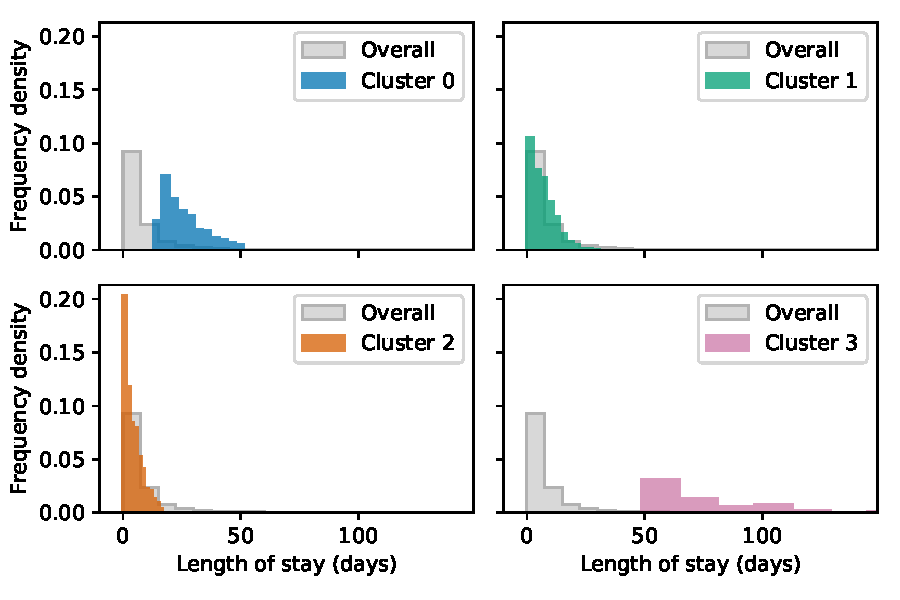
\includegraphics[width=\linewidth]{cluster_true_los}
        }\label{fig:cluster_los}
    }

    \subfloat[]{%
        \resizebox*{\imgwidth}{!}{%
            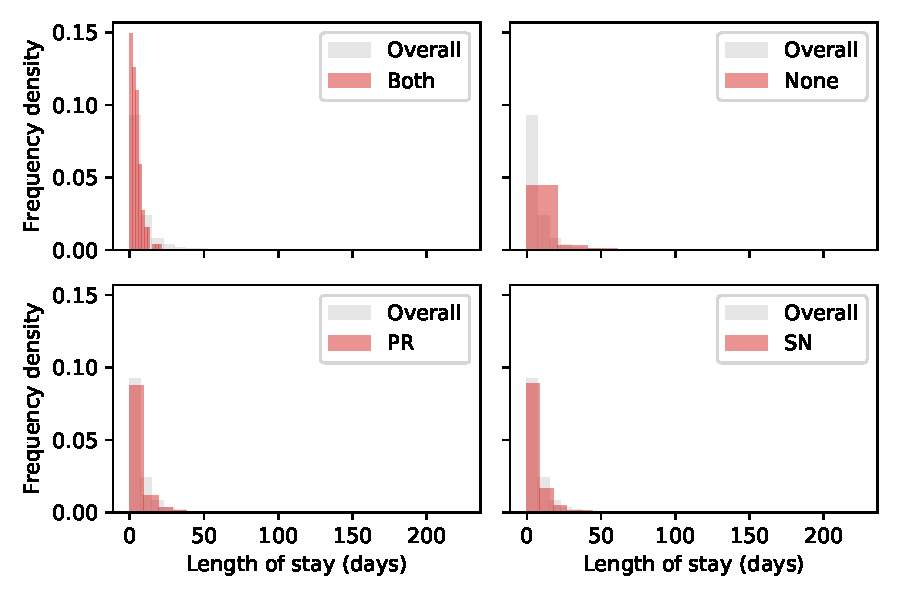
\includegraphics[width=\linewidth]{intervention_true_los}
        }\label{fig:intervention_los}
    }
    \caption{%
        Histograms for length of stay by~\subref{fig:cluster_los}~cluster
        and~\subref{fig:intervention_los}~intervention
    }
    \label{fig:los}
\end{figure}

\begin{figure}
    \centering
    \subfloat[]{%
        \resizebox*{\imgwidth}{!}{%
            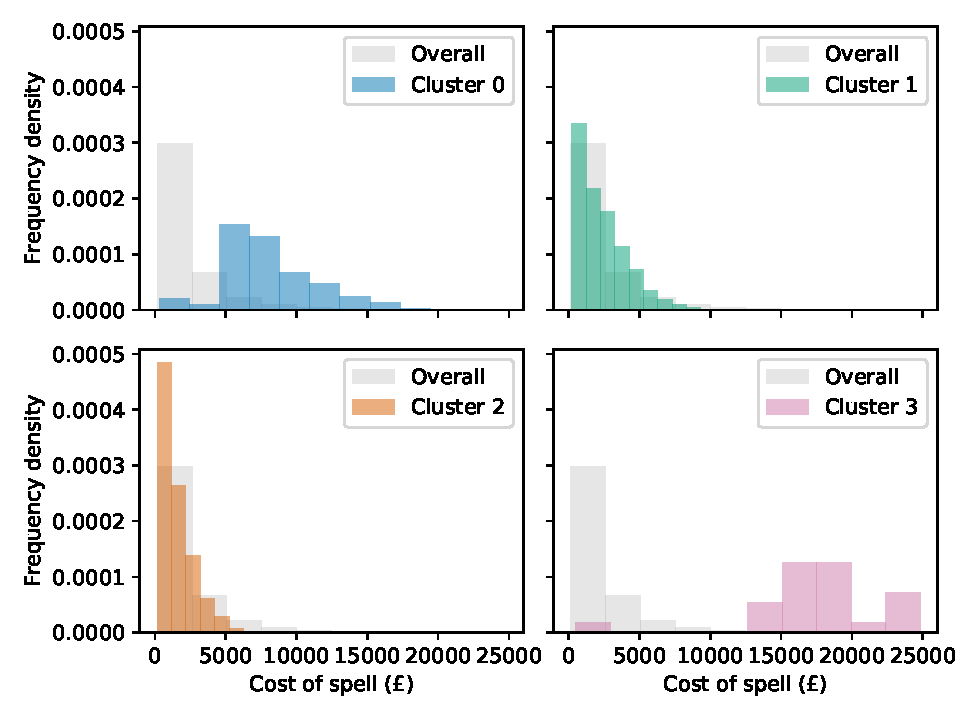
\includegraphics[width=\linewidth]{cluster_spell_cost}
        }\label{fig:cluster_cost}
    }

    \subfloat[]{%
        \resizebox*{\imgwidth}{!}{%
            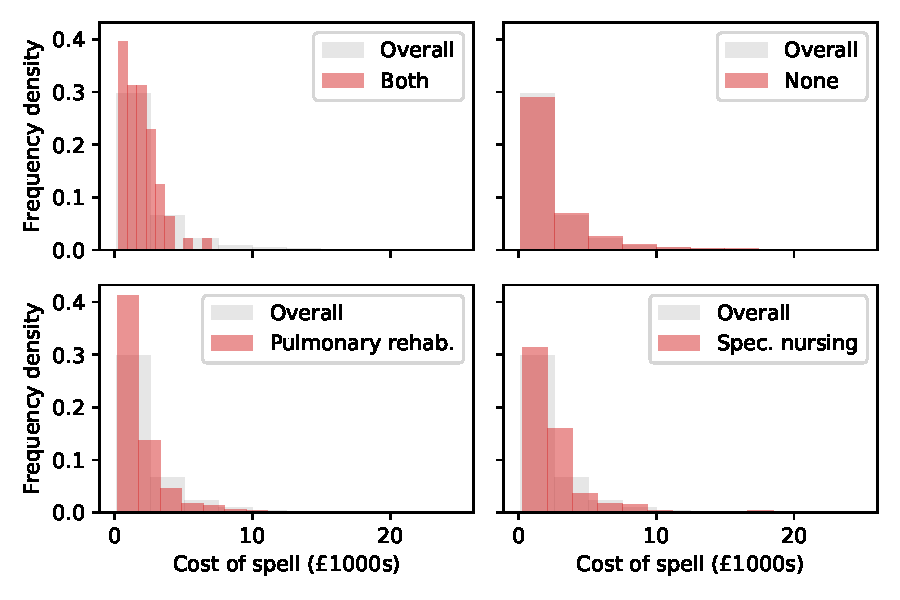
\includegraphics[width=\linewidth]{intervention_spell_cost}
        }\label{fig:intervention_cost}
    }
    \caption{%
        Histograms for spell cost by~\subref{fig:cluster_cost}~cluster
        and~\subref{fig:intervention_cost}~intervention
    }
    \label{fig:cost}
\end{figure}

Figure~\ref{fig:los} shows the length of stay distributions as histograms.
Figure~\ref{fig:cluster_los} demonstrates the different bed resource
requirements well for each cluster --- better than Table~\ref{tab:summary} might
--- in that the difference between the clusters is not only a matter of varying
means and ranges, but entirely different shapes to their respective
distributions. Indeed, they are all positively skewed, but there is no real
consistency beyond that. When comparing this to
Figure~\ref{fig:intervention_los}, there is undoubtedly some variety, but the
overall shapes of the distributions are generally similar. The exception is the
spells with no COPD intervention, where binning could not improve the
visualisation due to the widespread distribution of their lengths of stay.

The same conclusions can be drawn about spell costs from Figure~\ref{fig:cost};
there are distinct patterns between the clusters in terms of their costs, and
they align with the patterns seen in Figure~\ref{fig:los}. Such patterns are
expected given that length of stay is a driving force of healthcare costs.
Equally, there does not appear to be any immediately discernible difference in
the distribution of costs when splitting by intervention.

\begin{figure}
    \centering
    \subfloat[]{%
        \resizebox*{\imgwidth}{!}{%
            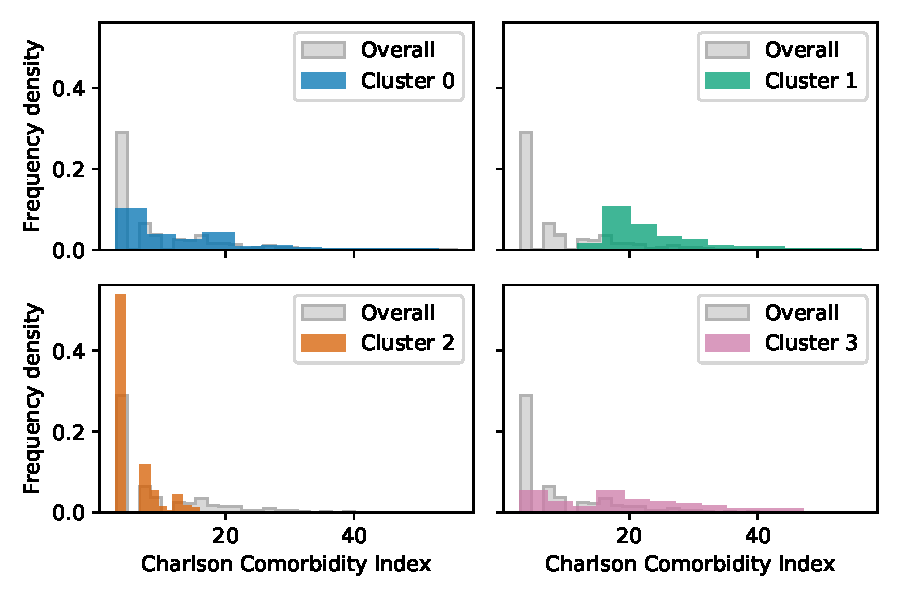
\includegraphics[width=\linewidth]{cluster_charlson_gross}
        }\label{fig:cluster_charlson}
    }

    \subfloat[]{%
        \resizebox*{\imgwidth}{!}{%
            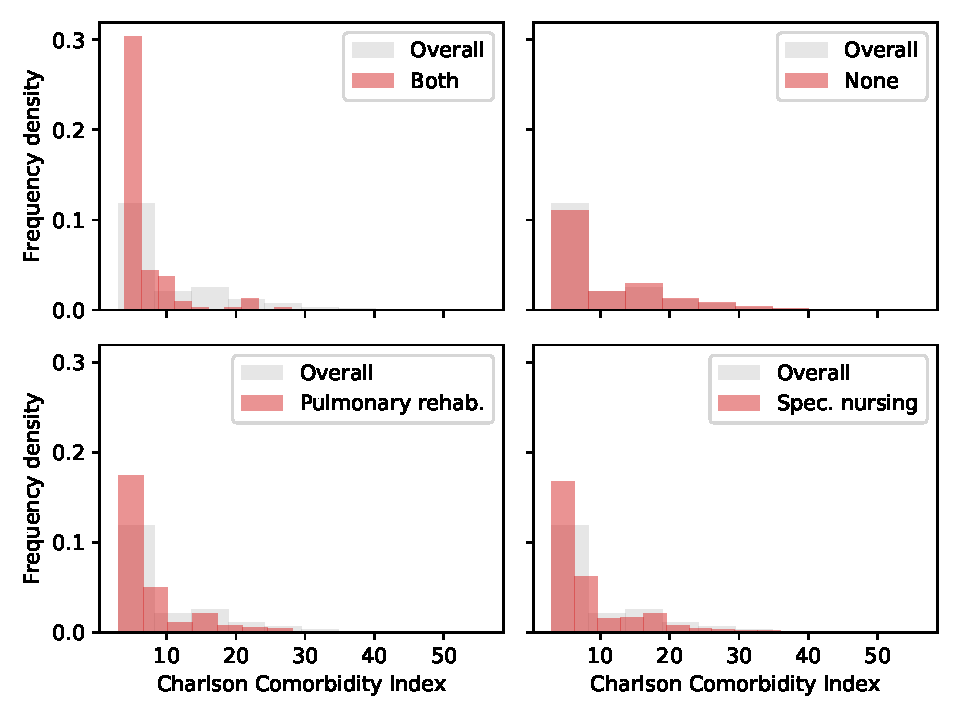
\includegraphics[width=\linewidth]{intervention_charlson_gross}
        }\label{fig:intervention_charlson}
    }
    \caption{%
        Histograms for CCI by~\subref{fig:cluster_charlson}~cluster
        and~\subref{fig:intervention_charlson}~intervention
    }\label{fig:charlson}
\end{figure}

Similarly to the previous figures, Figure~\ref{fig:charlson} shows that
clustering has revealed distinct patterns in the CCI of the spells within each
cluster, whereas splitting by intervention does not. All clusters other than
Cluster 2 show clear, heavy tails, and in the cases of Clusters 1 and 3, the
body of the data exists far from the origin as indicated in
Table~\ref{tab:summary}. In contrast, the plots in
Figure~\ref{fig:intervention_charlson} all display similar, highly skewed
distributions regardless of intervention.

\begin{figure}
    \centering
    \subfloat[]{%
        \resizebox*{\imgwidth}{!}{%
            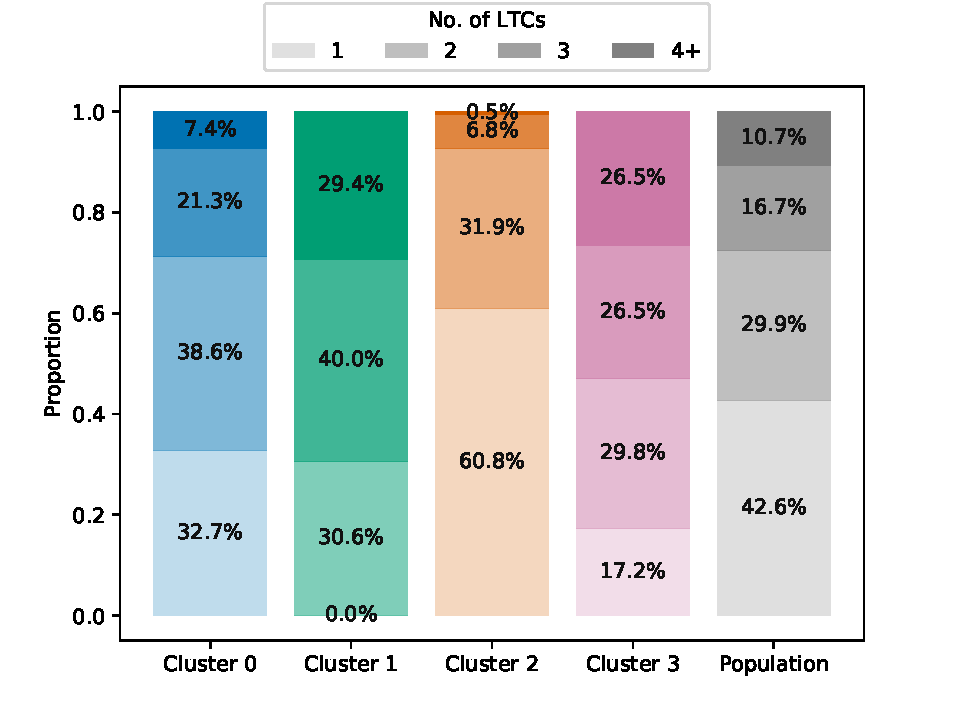
\includegraphics[width=\linewidth]{cluster_ltcs}
        }\label{fig:cluster_ltcs}
    }

    \subfloat[]{%
        \resizebox*{\imgwidth}{!}{%
            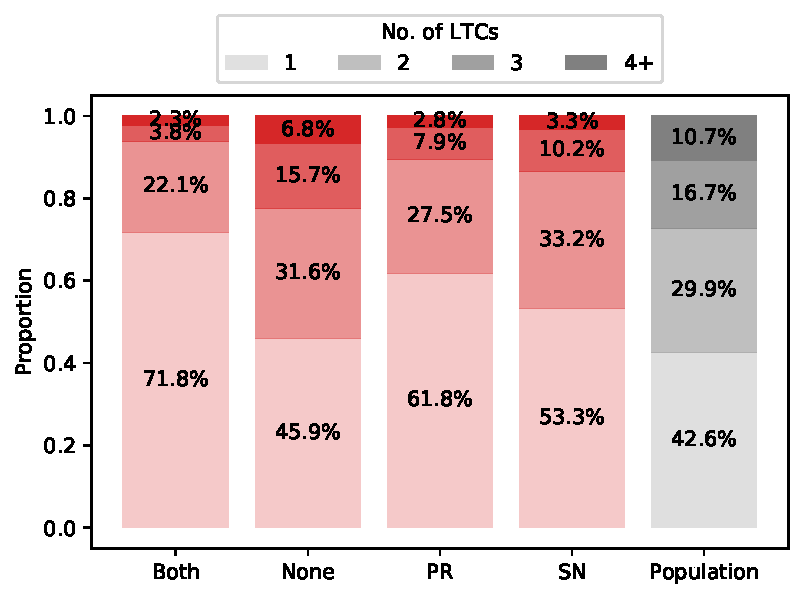
\includegraphics[width=\linewidth]{intervention_ltcs}
        }\label{fig:intervention_ltcs}
    }
    \caption{%
        Proportions of the number of concurrent LTCs in a spell
        by~\subref{fig:cluster_ltcs}~cluster
        and~\subref{fig:intervention_ltcs}~intervention
    }\label{fig:ltcs}
\end{figure}

\begin{figure}
    \centering
    \subfloat[]{%
        \resizebox*{\imgwidth}{!}{%
            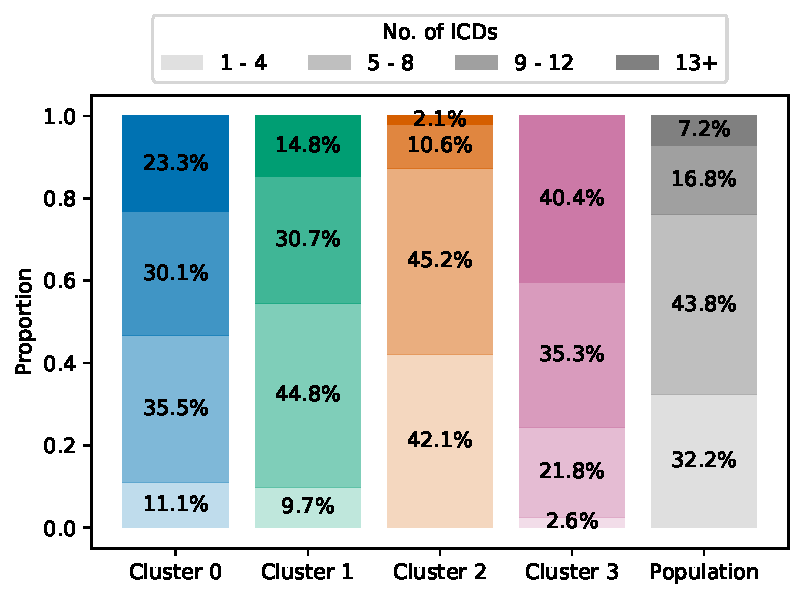
\includegraphics[width=\linewidth]{cluster_icds}
        }\label{fig:cluster_icds}
    }

    \subfloat[]{%
        \resizebox*{\imgwidth}{!}{%
            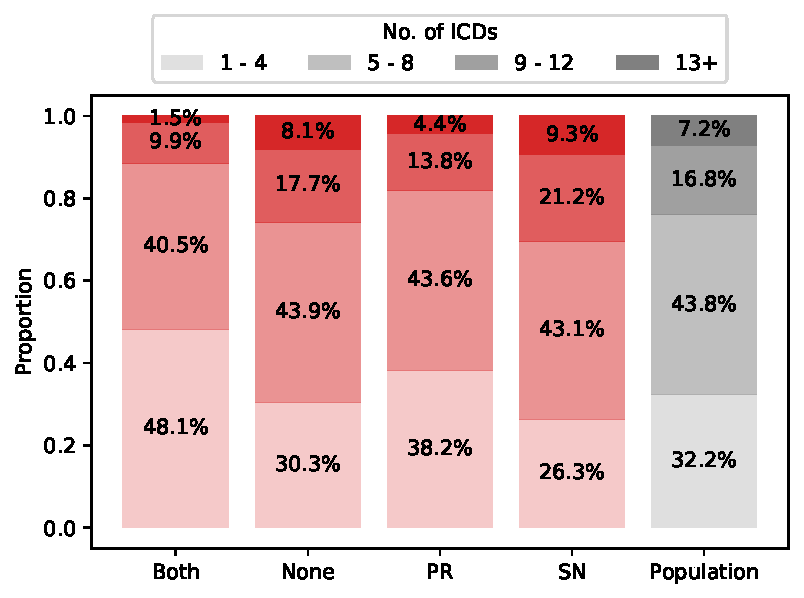
\includegraphics[width=\linewidth]{intervention_icds}
        }\label{fig:intervention_icds}
    }
    \caption{%
        Proportions of the number of concurrent ICDs in a spell
        by~\subref{fig:cluster_icds}~cluster
        and~\subref{fig:intervention_icds}~intervention
    }\label{fig:icds}
\end{figure}

Figures~\ref{fig:ltcs}~and~\ref{fig:icds} show the proportions of each grouping
presenting levels of concurrent LTCs and ICDs, respectively. By exposing the
distribution of these attributes, some notion of the clinical complexity for
each cluster can be captured better than with Table~\ref{tab:summary} alone. In
Figure~\ref{fig:cluster_ltcs}, for instance, there are distinct LTC count
profiles among the clusters: Cluster 0 is typical of the population; Cluster 1
shows that no patient presented COPD solely as an LTC in their spells, and more
than half presented at least three; Cluster 2 is similar in form to the
population but is strongly biased towards patients presenting COPD as the only
LTC; Cluster 3 has the closest-to-uniform spread among the four bins despite the
increased length of stay and CCI, suggesting a diverse array of patients in
terms of their long term medical needs.

Figure~\ref{fig:cluster_icds} largely mirrors these cluster profiles with the
number of concurrent ICDs. There are some points of interest, however. Firstly,
Cluster 1 has a relatively low-leaning distribution of ICDs that does not marry
up with the high rates of LTCs. Secondly, the vast majority of spells in Cluster
3 present with at least nine ICDs suggesting a likely wide range of conditions
and comorbidities beyond the LTCs used to calculate CCI.\

However, little can be drawn from the intervention counterparts to these figures
(i.e. Figures~\ref{fig:intervention_ltcs}~and~\ref{fig:intervention_icds}),
regarding the corresponding spells. One thing of note is that patients receiving
both interventions for their COPD (or either, in fact) have disproportionately
fewer LTCs and concurrent ICDs when compared to the population. Aside from this,
the profiles of each intervention are similar to one another.

As discussed earlier, the purpose of this manuscript is to construct a queuing
model for the data described here. Insights have already been gained into the
needs of the segments that have been identified in this section. However, to
glean further insights, some parameters of the queuing model must be recovered
from the data. The following section describes how these parameters are derived
using the dataset at hand.


\section{Constructing the queuing model}\label{sec:model}

The data available for study in this work is not as detailed as in comparative
projects. Without access to such data --- but intending to gain insight from
what is available --- it is imperative to bridge the gap left by the incomplete
data. Figure~\ref{fig:process} provides a diagrammatic depiction of the process
described in this section.

It is often the case that in practical situations where suitable data is not
(immediately) available, further inquiry in that line of research will stop.
Queuing models in healthcare settings appear to be such a case; the line ends at
incomplete queue data. The bibliographic work~\cite{Asanjarani2017} collates
articles on the estimation of queuing system characteristics --- including their
parameters. Despite its breadth of almost 300 publications from 1955, only two
articles have been identified as being applied to
healthcare:~\cite{Mohammadi2012,Yom2014}. Both works are concerned with
customers who can re-enter services during their time in the queuing system,
which is mainly of value when considering the effect of unpredictable behaviour
in intensive care units, for instance. In~\cite{Mohammadi2012}, the authors seek
to approximate service and re-service densities through a Bayesian approach and
by filtering out those customers seeking to be serviced again. Meanwhile, the
approach in~\cite{Yom2014} considers an extension to the \(M/M/c\) queue with
direct re-entries. The devised model is then used to determine resource
requirements in two healthcare settings.

Aside from healthcare-specific works, the approximation of queue parameters has
formed a part of relevant modern queuing research. However, the scope is
primarily focused on theoretic approximations rather than simulation. For
instance, two recent works~\citep{Djabali2018,Goldenshluger2016}, consider an
underlying process to estimate a general service time distribution in single
server and infinite server queues respectively.

While these solutions are interesting, they do not necessarily tackle the issue
in this scenario where information about the system is also missing. With that,
there is a precedent for simplifying healthcare systems to a single node with
parallel servers that emulate overall resource availability. Two
studies~\citep{Steins2013,Williams2015}, provide examples of how this approach,
when paired with discrete event simulation, can expose the resource needs of a
system beyond deterministic queuing theory models. In particular, the authors
of~\cite{Williams2015} show how a single node, multiple server queue can be used
to accurately predict bed capacity and length of stay distributions in a
critical care unit using administrative data.

\begin{figure}
    \centering%
    \resizebox{!}{.9\textheight}{\usepackage{amsmath}
    \DeclareMathOperator*{\argmin}{arg\,min}

\usepackage{tikz}
    \usetikzlibrary{%
        arrows,
        backgrounds,
        decorations.pathreplacing,
        shapes.geometric,
        positioning,
    }

\definecolor{blue}{HTML}{0072B2}
\definecolor{green}{HTML}{009E73}
\definecolor{orange}{HTML}{D55E00}
\definecolor{pink}{HTML}{CC79A7}

\pgfdeclarelayer{background}
\pgfsetlayers{background,main}

\tikzstyle{every picture} += [remember picture]
\tikzstyle{na} = [baseline=-.5ex]

\tikzset{%
    queue/.pic={%
        code{%
            \node (rect) at (38.5mm, 10mm) {};
            \draw[thick] (0, 0) -- ++(40mm, 0) -- ++(0, 20mm) -- ++(-40mm, 0);
            \foreach \val in {0, ..., #1}{%
                \draw[thick] ([xshift=-\val*5mm] 40mm, 20mm) -- ++(0, -20mm);
            };

            \foreach \val/\lab/\size in {%
                0/1/\scriptsize,
                1/2/\scriptsize,
                3/c-1/\tiny,
                4/c/\scriptsize%
            }{%
                \node[draw, circle, thick, minimum size=9.5mm] (\lab)
                    at (55mm, 29mm - \val * 9.5mm) {\size$\lab$};
                \draw[-latex, thick] (rect.east) -- (\lab.west);
            };
            
            \node at (55mm, 11mm) {$\vdots$};
            \node at (5mm, 10mm) {$\cdots$};
        };
    },
    myarrow/.style={%
        line width=2mm,
        draw=gray!50,
        -triangle 60,
        postaction={draw=gray!50, line width=4mm, shorten >=6mm, -},
    },
    double -latex/.style args={#1 colored by #2 and #3}{%
        -latex,
        line width=#1,
        #2,
        postaction={%
            draw,
            -latex,
            #3,
            line width=(#1)/3,
            shorten <=(#1)/4,
            shorten >=4.5*(#1)/3
        },
    },
    mypointer/.style={%
        double -latex=1mm colored by gray!50 and gray!50,
    }
}
}
    \caption{%
        A diagrammatic depiction of the queuing parameter recovery process
    }\label{fig:process}
\end{figure}

The \(M/G/c\) queue cannot be represented as a Markov chain, but it is a
stochastic process on the same state space as the other queues in this section.
Given the generic nature of customer departure times, a lot of the structure of
the underlying process is lost. As such, deriving exact values for many
properties of the \(M/G/c\) queue continues to be an open
problem~\citep{Kingman2009}. Despite the theoretical challenges posed by the
\(M/G/c\) queue, simulating these generic queues can still be of great benefit
--- as is done in Section~\ref{sec:model}. 

\subsection{Deriving the model parameters}\label{subsec:derive}

Following in the suit of recent literature~\citep{Steins2013,Williams2015}, this
work employs a single node using the \(M/G/c\) queue to model a hypothetical
ward of patients presenting COPD.\ In addition to this, the grouping found in
Section~\ref{subsec:overview} provides a set of patient classes in the queue.
Under this model, the following assumptions are made:

\begin{enumerate}
    \item Inter-arrival and service times of patients are each exponentially
        distributed with some mean. This distribution is used to simplify the
        model parameterisation.
    \item There are \(c \in \mathbb{N}\) servers available to arriving patients
        at the node representing the overall resource availability, including
        bed capacity and hospital staff.
    \item There is no queue or system capacity. In~\cite{Williams2015}, a
        queue capacity of zero is set under the assumption that any surplus
        arrivals would be sent to another suitable ward or unit. As this
        hypothetical ward represents the sole unit for COPD patients within the
        health board, this assumption is not held.
    \item Without the availability of expert clinical knowledge, a
        first-in-first-out service policy is employed in place of some patient
        priority framework.
\end{enumerate}

Each group of patients has its arrival distribution, the parameter of which is
the reciprocal of the mean inter-arrival times for that group. This parameter
is denoted by \(\lambda_l\) for each cluster \(l\).

Like arrivals, each group of patients has its service time distribution.
Without full details of the process order or idle periods during a spell, some
assumption must be made about the actual `service' time of a patient in the
hospital. It is assumed here that the mean service time of a group of patients
may be approximated via their mean length of stay, i.e. the mean time spent in
the system. As indicated by the distributions in Figure~\ref{fig:cluster_los},
the length of stay distributions require shifting prior to fitting an
exponential distribution.

Let \(T_l\) denote the set of observed lengths of stay for cluster \(l\), and
let \(m_l = \max \left\{0, \min T_l\right\}\) be its feasible minimum. Thus, the
\emph{shifted times} for cluster \(l\), denoted \(\widehat T_l\), are:

\begin{equation}\label{eq:shifted}
    \widehat T_l := \left\{t - m_l : t \in T_l\right\}
\end{equation}

An exponential distribution may be fitted to these shifted system times by
using their mean, denoted by \(\frac{1}{\phi_l}\), as the distribution
parameter. For the sake of simplicity, it is assumed that for each cluster
\(l\), the mean shifted service time of that cluster, \(\frac{1}{\mu_l}\), is
proportional to the corresponding mean shifted system time such that:

\begin{equation}\label{eq:shifted_services}
    \mu_l = p_l \phi_l
\end{equation}

\noindent where \(p_l \in \interval[open left]{0}{1}\) is a {\slshape service
proportion} parameter to be determined for each group.

With these definitions, the service time for cluster \(l\), denoted \(S_l\), is
distributed by a {\slshape shifted exponential distribution} with a mean of
\(\frac{1}{\mu_l}\) and shift of \(m_l\). The probability density function
of this distribution is as follows:

\begin{equation}\label{eq:shifted_pdf}
    f(s) = \begin{cases}
        \mu_l e^{-\mu_l (s - m_l)} & \quad \text{if \(s \ge m_l\)}\\
        0 & \quad \text{otherwise}
    \end{cases}
\end{equation}

Since this distribution is geometrically identical to the exponential
distribution with rate \(\mu_l\) except for a shift of \(m_l\), its memoryless
property holds for \(s \ge m_l\). However, since this model allows for multiple
classes and the shift terms are not the same for each cluster, this model
technically should be reclassified as a \(M/G/c\) model. Regardless of this, the
mean service time for spells in cluster \(l\) is given by:

\begin{equation}\label{eq:services}
    \mathbb E \left(S_l\right)
    = \int_{m_l}^{\infty} \mu_l s e^{-\mu_l (s - m_l)} \mathrm ds
    = m_l + \frac{1}{\mu_l}
\end{equation}

\subsection{Validating the model}\label{subsec:validate}

One of the few ground truths available in the provided data is the observed
length of stay distribution. Given that the length of stay and resource
availability are connected, the approach here will be to simulate the length of
stay distributions for a range of values \(p_l\) and \(c\), to find the
parameters that best match the observed data.

Several methods are available for the statistical comparison of two or more
distributions, such as the Kolmogorov-Smirnov test, a variety of discrepancy
approaches such as summed mean-squared error, and \(f\)-divergences. A popular
choice among the last group (which may be considered distance-like) is the
Kullback-Leibler divergence which measures relative information entropy from one
probability distribution to another~\citep{Kullback1951}. A key issue with many
of these methods is that they lack interpretability, something which is
paramount when conveying information to stakeholders, not only for explaining
how something works, but also how its results may be explained.

As such, a reasonable candidate is the (first) Wasserstein metric, also known as
the `earth mover' or `digger' distance~\citep{Vaserstein1969}. The Wasserstein
metric satisfies the conditions of a formal mathematical metric --- like
Euclidean distance or the dissimilarity measure given in
Definition~\ref{def:dissim}. Also, the values of the Wasserstein metric take the
units of the distributions under comparison (in this case: days). These
characteristics can aid understanding and explanation. The distance measures the
approximate `minimal work' required to move between two probability
distributions where `work' can be loosely defined as the product of how much of
the distribution's mass moves and the distance by which it must be moved. More
formally, the Wasserstein distance between two probability distributions \(U\)
and \(V\) is defined as:

\begin{equation}\label{eq:wasserstein}
    W(U, V) = \int_{0}^{1} \left\vert F^{-1}(t) - G^{-1}(t) \right\vert dt
\end{equation}

Here, \(F\) and \(G\) are the cumulative density functions of \(U\) and \(V\),
respectively. A proof of~\eqref{eq:wasserstein} is presented
in~\cite{Ramdas2017}.

Each trial used here takes a parameter set and simulates the ward across a
series of independent repetitions. The parameter set with the smallest maximum
distance between the simulated system time distribution and the observed length
of stay distribution is taken to be the most appropriate. To be specific, let
\(T_{c,p}\) denote the system time distribution obtained from a simulation with
\(c\) servers and \(p := \left(p_0,p_1,p_2,p_3\right)\), and let \(T\) denote
the observed length of stay distribution. Then the optimal parameter set
\(\left(c^*, p^*\right)\) is given by:

\begin{equation}\label{eq:parameters}
    \left(c^*, p^*\right) = \argmin_{c, p} \left\{%
        \max \left\{ W\left(T_{c,p}, T\right) \right\}%
    \right\}
\end{equation}

The parameter sweep included values of each \(p_l\) from \(0.5\) to \(1.0\) with
a granularity of \(5.0 \times 10^{-2}\) and values of \(c\) from \(30\) to
\(50\) at steps of five. These choices were informed by the assumptions of the
model and formative analysis to reduce the parameter space given the
computational resources required to conduct the simulations. Each parameter set
was repeated 50 times, with each simulation running for four years of virtual
time. The warm-up and cool-down periods were taken to be approximately one year
each, leaving two years of simulated data from each repetition.

\begin{figure}
    \centering
    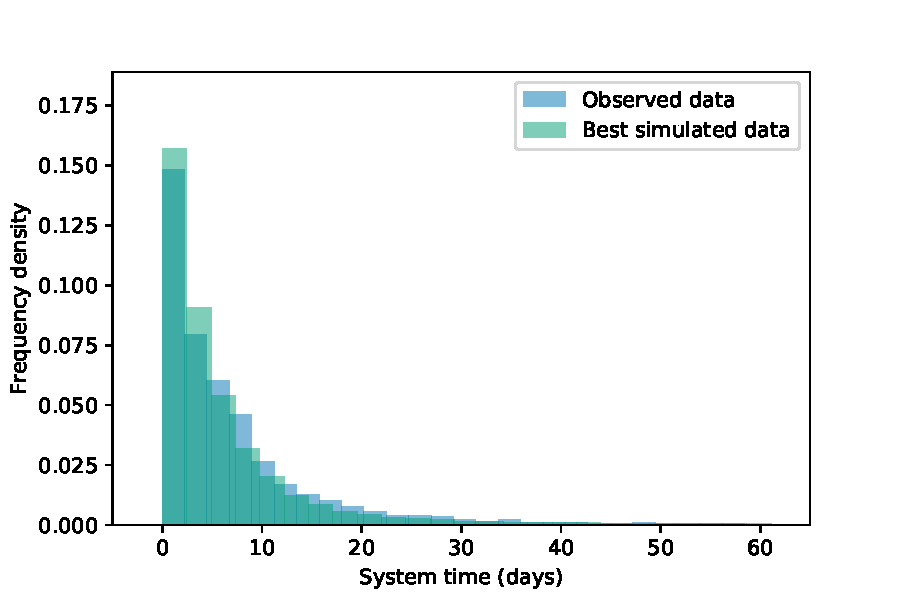
\includegraphics[width=\imgwidth]{best_params}
    \caption{%
        Histograms of the best-simulated and observed LOS data
    }\label{fig:best_params}
\end{figure}

\begin{figure}
    \centering
    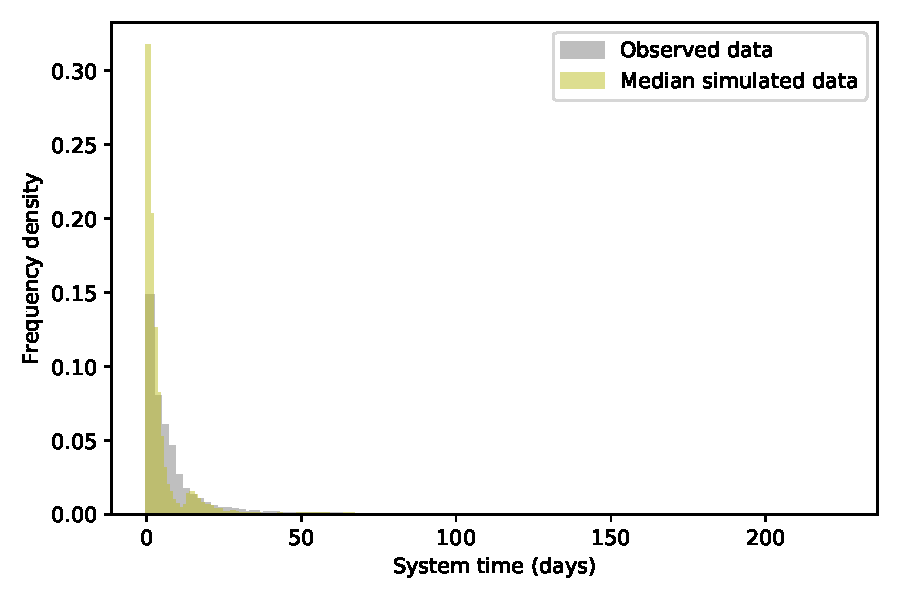
\includegraphics[width=\imgwidth]{median_params}
    \caption{%
        Histograms of the median-simulated and observed LOS data
    }\label{fig:median_params}
\end{figure}

\begin{figure}
    \centering
    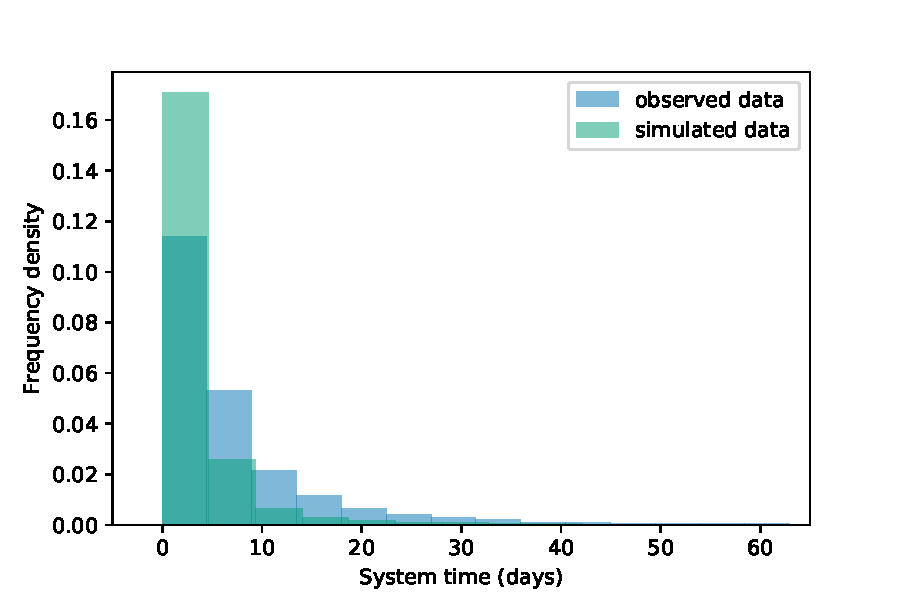
\includegraphics[width=\imgwidth]{worst_params}
    \caption{%
        Histograms of the worst-simulated and observed LOS data
    }\label{fig:worst_params}
\end{figure}

The results of this parameter sweep are summarised in
Figures~\ref{fig:best_params}~through~\ref{fig:worst_params}. Each plot shows a
comparison of the observed lengths of stay across all groups and the newly
simulated data with the best, median and worst parameter sets, respectively.
These figures highlight the importance of choosing good parameters under this
model as the differences in the quality of the fits are stark. In the best case
the fit is uncanny, whereas the median case shows a distribution that inflates
the presence of short-stay patients despite an otherwise good fit. Meanwhile,
Figure~\ref{fig:worst_params} displays a distribution that only resembles the
observed distribution in its positive skew; the worst-case distribution lacks
the distinctive `exponential' nose and has a considerably heavier tail
corresponding to a disproportionate amount of long-stay patients.
Table~\ref{tab:comparison} reinforces these results numerically, showing a
precise fit by the best parameter set across all measures, except the maximum
recorded stay.

\begin{table}
    \centering
    \resizebox{\textwidth}{!}{\begin{tabular}{lrrrrrrrrrrrrr}
\toprule
{} & \multicolumn{6}{l}{Model parameter and result} & \multicolumn{7}{l}{LOS statistic} \\
{} &                    \(p_0\) & \(p_1\) & \(p_2\) & \(p_3\) & \(c\) & Max. distance &          Mean &   Std. &  Min. &   25\% &  Med. &   75\% &    Max. \\
\midrule
Observed        &                        NaN &     NaN &     NaN &     NaN &   NaN &          0.00 &          7.70 &  11.86 & -0.02 &  1.49 &  4.20 &  8.93 &  224.93 \\
Best simulated  &                        1.0 &     1.0 &     1.0 &     0.5 &  50.0 &          1.30 &          7.11 &  12.41 &  0.00 &  1.44 &  3.55 &  7.64 &  244.46 \\
Worst simulated &                        0.5 &     0.5 &     0.5 &     1.0 &  40.0 &          4.25 &          4.36 &  13.40 &  0.00 &  0.72 &  1.78 &  3.84 &  463.01 \\
\bottomrule
\end{tabular}
}
    \caption{%
        A comparison of the observed and simulated data based on the model
        parameters and summary statistics for length of stay
    }\label{tab:comparison}
\end{table}

In this section, the previously identified clustering enriched the overall
queuing model and was used to recover the parameters for several classes within
that. Now, using this model, the next section details an investigation into the
underlying system by adjusting the parameters of the queue with the clustering.

\section{Adjusting the queuing model}\label{sec:scenarios}

This section comprises several what-if scenarios --- a classic component of
healthcare operational research --- under the novel parameterisation of the
queue established in Section~\ref{sec:model}. The outcomes of interest in this
work are server (resource) utilisation and system times. These metrics capture
the driving forces of cost and the state of the system. Specifically, the
objective of these experiments is to address the following questions:
\begin{itemize}
    \item How is the system affected by a change in overall patient arrivals?
    \item How is the system affected by a change in resource availability?
    \item How is the system affected by patients moving between clusters?
\end{itemize}

Given the nature of the observed data, the queuing model parameterisation and
its assumptions, the effects on the chosen metrics in each scenario are in
relative terms with respect to the base case. The base case being those results
generated from the best parameter set recorded in Table~\ref{tab:comparison}. In
particular, the data from each scenario is scaled by the corresponding median
value in the base case, meaning that a metric having a value of 1 is `normal'.

As mentioned in Section~\ref{sec:intro}, the source code used throughout
this manuscript has been archived online under~\doi{10.5281/zenodo.4457902}.
Also, the datasets generated from the simulations in this section, and the
parameter sweep, have been archived online~\doi{10.5281/zenodo.4457808}.


\subsection{Changes to overall patient arrivals}\label{subsec:arrivals}

Changes in overall patient arrivals to a queue reflect real-world scenarios
where some stimulus is improving (or worsening) the condition of the patient
population. Examples of stimuli could include an ageing population or
independent life events that lead to a change in deprivation, such as an
accident or job loss. Within this model, overall patient arrivals are altered
using a scaling factor denoted by \(\sigma > 0\). This scaling factor is applied
to the model by multiplying each cluster's arrival rate by \(\sigma\). That is,
the new arrival rate for a cluster, \(l\), denoted \(\hat\lambda_l\), is given
by:

\begin{equation}\label{eq:lambda}
    \hat\lambda_{l} = \sigma\lambda_l
\end{equation}

\begin{figure}
    \centering
    \subfloat[]{%
        \resizebox*{\imgwidth}{!}{%
            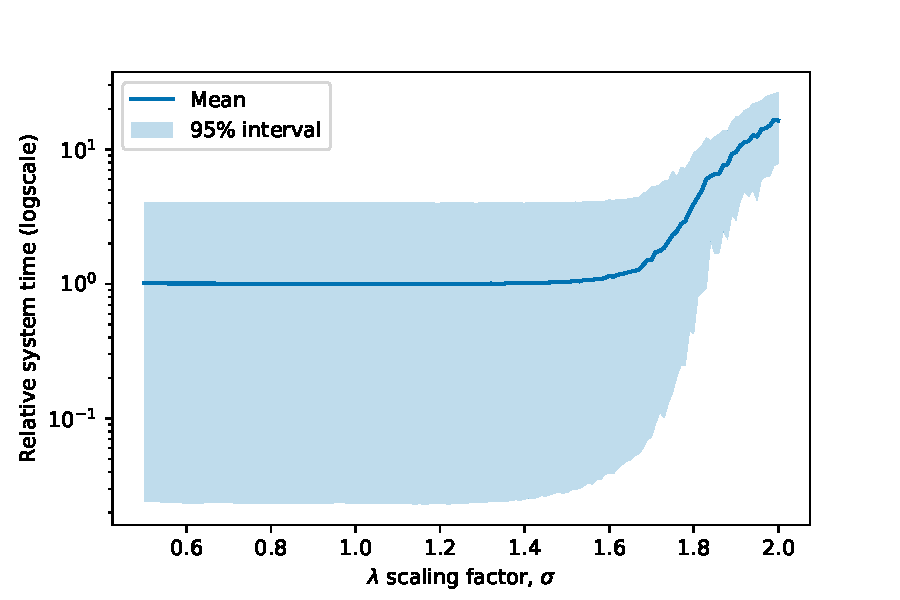
\includegraphics[width=\linewidth]{lambda_time}
        }\label{fig:lambda_time}
    }

    \subfloat[]{%
        \resizebox*{\imgwidth}{!}{%
            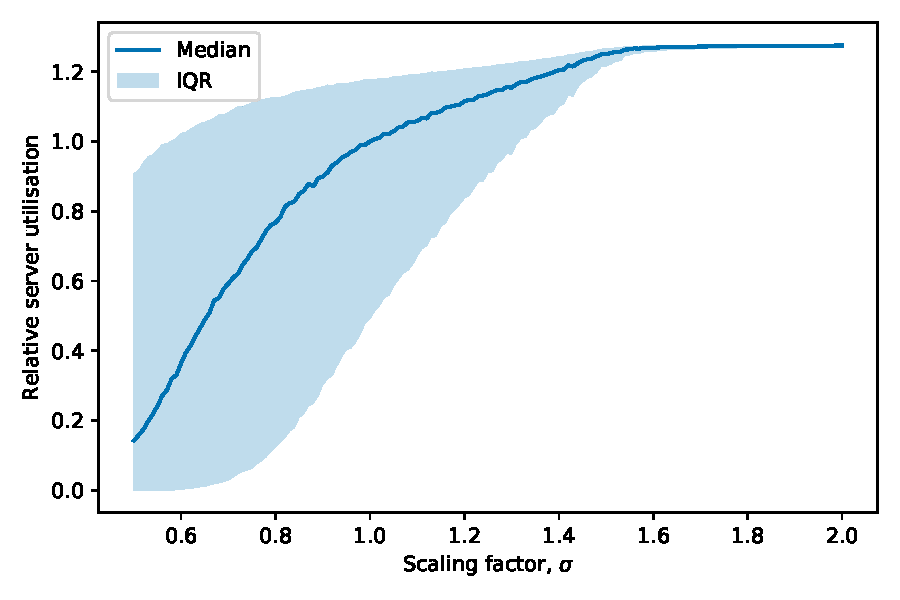
\includegraphics[width=\linewidth]{lambda_util}
        }\label{fig:lambda_util}
    }
    \caption{%
        Plots of \(\sigma\) against relative
        \subref{fig:lambda_time}~system~time and
        \subref{fig:lambda_util}~server~utilisation
    }\label{fig:lambda}
\end{figure}

Figure~\ref{fig:lambda} shows the effects of changing patient arrivals on
(\subref{fig:lambda_time})~relative system times and
(\subref{fig:lambda_util})~relative server utilisation for values of \(\sigma\)
from 0.5 to 2.0 at a precision of \(1.0 \times 10^{-2}\). Specifically, each
plot in the figure (and the subsequent figures in this section) shows the median
and interquartile range (IQR) of each relative attribute. These metrics provide
an insight into the experience of a typical user (or server) in the system.
Furthermore, they reveal the stability and variation of the body of users
(or servers).

What is evident from these plots is that things are happening as one might
expect: as arrivals increase, the strain on the system increases. However, it
should be noted that it also appears that the model has some amount of slack
relative to the base case. Looking at Figure~\ref{fig:lambda_time}, for
instance, the relative system time distribution stays unchanged up to \(\sigma
\approx 1.2\), or an approximate 20\% increase in arrivals of COPD patients.
Beyond that, relative system times quickly rise to an untenable point where the
median time becomes orders of magnitude above the norm.

However, Figure~\ref{fig:lambda_util} shows that the situation for the system's
resources reaches its worst-case near to the start of that spike in relative
system times (at \(\sigma \approx 1.3\)). That is, the median server utilisation
reaches a maximum (this corresponds to constant utilisation) at this point, and
the variation in server utilisation disappears entirely. The reality of this
situation is that the system has no slack at all, and all parts of the system
are under equal load, which is not preferable given the differences in resource
requirements for the parts of a hospital system. For instance, if surgical
theatres were in constant use but administrative processing required an
equivalent amount of resources to continue running, the system would likely
falter or deteriorate entirely.


\subsection{Changes to resource availability}\label{subsec:resources}

As is discussed in Section~\ref{sec:model}, the resource availability of the
system is captured by the number of parallel servers, \(c\). Therefore, to
modify the overall resource availability, only the number of servers needs to be
changed. This kind of sensitivity analysis is usually done to determine the
opportunity cost of adding service capacity to a system, e.g.\ would an increase
of \(n\) servers sufficiently increase efficiency without exceeding a budget?

To reiterate the beginning of this section: all suitable parameters are given in
relative terms, including the number of servers here. By doing this, the changes
in resource availability are more evident, and do away with any concerns as to
what a particular number of servers precisely reflects in the real world, be it
any combination of hospital beds, equipment availability and medical staff.

% \begin{figure}
%     \centering
%     \begin{subfigure}{\imgwidth}
%         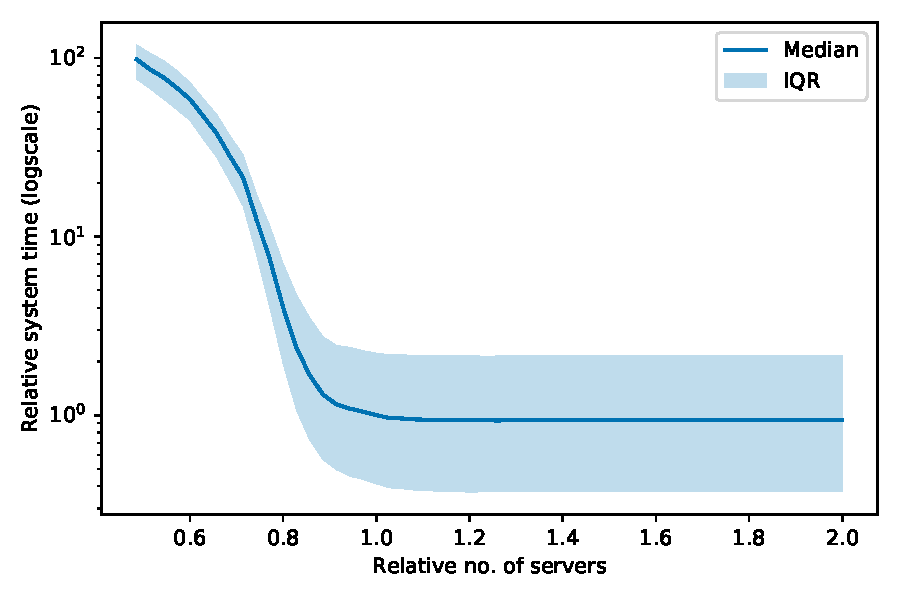
\includegraphics[width=\linewidth]{servers_time}
%         \caption{}\label{fig:servers_time}
%     \end{subfigure}

%     \begin{subfigure}{\imgwidth}
%         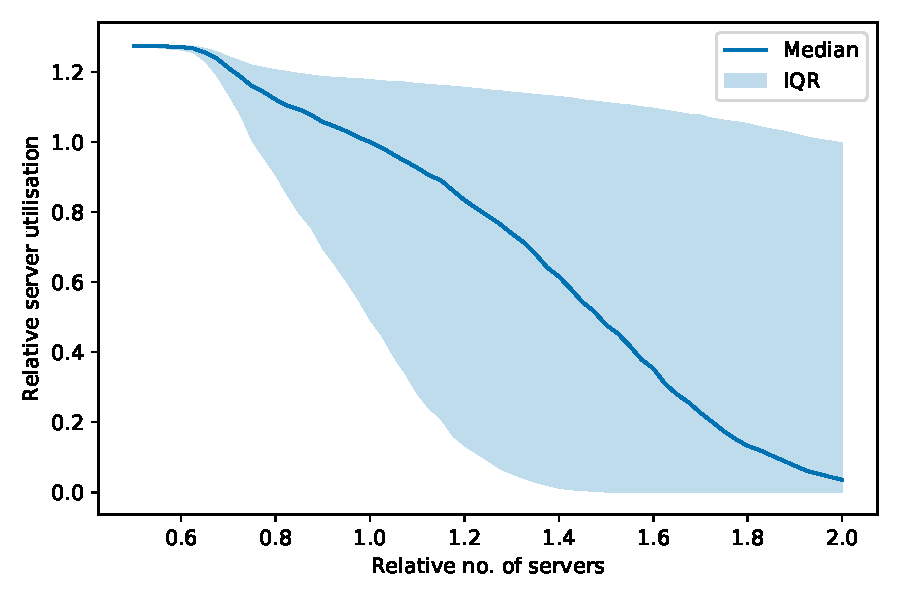
\includegraphics[width=\linewidth]{servers_util}
%         \caption{}\label{fig:servers_util}
%     \end{subfigure}
%     \caption{%
%         Plots of the relative number of servers against relative
%         (\subref{fig:servers_time})~system time and
%         (\subref{fig:servers_util})~server utilisation
%     }\label{fig:servers}
% \end{figure}

Figure~\ref{fig:servers} shows how the relative resource availability affects
relative system times and server utilisation. In this scenario, the relative
number of servers took values from 0.5 to 2.0 at an equivalent step size of one
in the number of servers, i.e. \(c\) takes values from 17 to 70. Overall, these
figures fortify the claim from the previous scenario that there is some room to
manoeuvre so that the system runs `as normal', but pressing on those boundaries
results in massive changes to both resource requirements and system times.

In Figure~\ref{fig:servers_time} this amounts to a maximum of 10\% slack in
resources before relative system times are substantially affected; further
reductions quickly result in a potentially tenfold increase in the median system
time, and up to 100 times once resource availability falls by 50\%. Moreover,
the variation in the body of the relative times (i.e. the IQR) decreases as
resource availability decreases. The reality of this is that patients arriving
at a hospital are forced to consume more significant amounts of resources (by
merely being in a hospital) regardless of their condition, putting added strains
on the system. Figure~\ref{fig:servers_util} mirrors these observations on the
small amount of slack in resource requirements, but (as with the previous
scenario) constant utilisation occurs quickly.

Meanwhile, it appears that there is no tangible change in relative system times
given an increase in the number of servers. This indicates that the model
carries sufficient resources to cater to the population under normal
circumstances and that adding service capacity will not necessarily improve
system times.

Again, Figure~\ref{fig:servers_util} shows that there is a substantial change in
the variation in the relative utilisation of the servers. In this case, the
variation dissipates as resource levels fall, and increases as resources
increase. While the relationship between real hospital resources and the number
of servers is not exact, having variation in server utilisation would suggest
that small parts of an existing system may be configured or partitioned away in
the case of some significant public health event (such as a global pandemic)
without overloading the system.


\subsection{Moving arrivals between clusters}\label{subsec:moving}

This scenario is perhaps the most relevant to actionable public health research
of those presented here. The clusters identified in this work could be
characterised by their clinical complexities and resource requirements, as done
in Section~\ref{subsec:overview}. Therefore, being able to model the movement of
some proportion of patient spells from one cluster to another will reveal how
those complexities and requirements affect the system itself. The reality is
then that if some public health policy could be implemented to initiate that
movement informed by a model such as this, then change would be seen in the real
system.

In order to model the effects of spells moving between two clusters, the
assumption is that each cluster's service time distribution stays the same (and
so does each cluster's \(p_l\)), but their arrival rates are altered according
to some transfer proportion. Consider two clusters indexed at \(l\) and \(m\),
and their respective arrival rates, \(\lambda_l\), \(\lambda_m\). Let \(\delta
\in [0, 1)\) denote the proportion of arrivals to be moved from cluster \(l\) to
cluster \(m\). Then the new arrival rates for each cluster, denoted by
\(\hat\lambda_l, \hat\lambda_m\) respectively, are:

\begin{equation}\label{eq:moving}
    \hat\lambda_l = \left(1 - \delta\right) \lambda_l
    \quad \text{and} \quad
    \hat\lambda_m = \delta\lambda_l + \lambda_m
\end{equation}

By moving patient arrivals between clusters in this way, the overall arrivals
are left the same since the sum of the arrival rates is the same. Hence, the
(relative) effect on server utilisation and system time can be measured
independently.

Figures~\ref{fig:moving_time}~and~\ref{fig:moving_util} show the effect on
relative system time and relative server utilisation, respectively, of moving
patient arrivals between clusters. In each figure, the median and IQR for the
corresponding attribute is shown, as in the previous scenarios. Each scenario
was simulated using values of \(\delta\) from 0.0 to 0.98 at steps of \(2.0
\times 10^{-2}\).

\begin{figure}
    \centering
    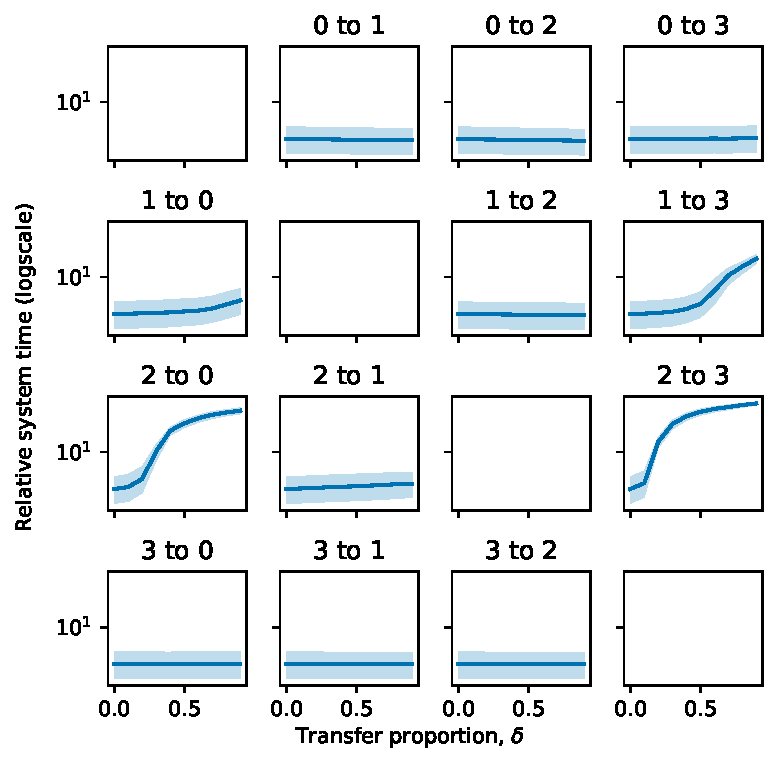
\includegraphics[width=\textwidth]{moving_time}
    \caption{%
        Plots of proportions of each cluster moving to another against relative
        system time
    }\label{fig:moving_time}
\end{figure}

\begin{figure}
    \centering
    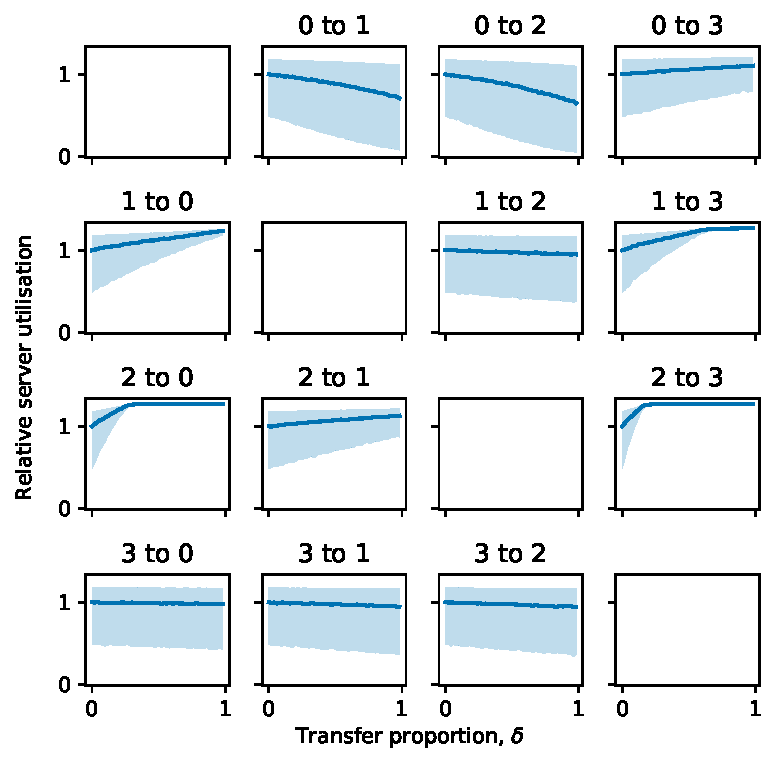
\includegraphics[width=\textwidth]{moving_util}
    \caption{%
        Plots of proportions of each cluster moving to another on relative
        server utilisation
    }\label{fig:moving_util}
\end{figure}

Considering Figure~\ref{fig:moving_time}, it appears that each type of transfer
falls into one of two categories: either completely derailing the system (such
as moving any cluster to Cluster 3) or improving system times, albeit mildly. 
The latter case occurs in the following transfers:

\begin{itemize}
    \item Cluster 0 to Clusters 1 or 2
    \item Cluster 1 to Cluster 2
    \item Cluster 3 to any other cluster
\end{itemize}

A finer look at the effect of these transfer types on relative system times is
given in Table~\ref{tab:moving_time}. Likewise, their effects on relative server
utilisation is given in Table~\ref{tab:moving_util}. 

\begin{table}
    \centering%
    \resizebox{\textwidth}{!}{\begin{tabular}{llrrrrrrrrrr}
\toprule
    & \textbf{\(\delta\)} &  0.0 &     0.1 &     0.2 &     0.3 &     0.4 &     0.5 &     0.6 &     0.7 &     0.8 &     0.9 \\
\textbf{Origin} & \textbf{Destination} &      &         &         &         &         &         &         &         &         &         \\
\midrule
\textbf{0} & \textbf{1} &  0.0 & -0.0268 & -0.0582 & -0.0847 & -0.1048 & -0.1160 & -0.1289 & -0.1416 & -0.1544 & -0.1641 \\
  & \textbf{2} &  0.0 & -0.0522 & -0.0701 & -0.0930 & -0.1175 & -0.1383 & -0.1523 & -0.1665 & -0.1827 & -0.1955 \\
\textbf{1} & \textbf{2} &  0.0 & -0.0203 & -0.0385 & -0.0470 & -0.0585 & -0.0763 & -0.0858 & -0.0956 & -0.0921 & -0.1193 \\
\textbf{3} & \textbf{0} &  0.0 & -0.0177 & -0.0282 & -0.0274 & -0.0259 & -0.0365 & -0.0376 & -0.0541 & -0.0475 & -0.0554 \\
  & \textbf{1} &  0.0 & -0.0309 & -0.0362 & -0.0320 & -0.0431 & -0.0570 & -0.0634 & -0.0633 & -0.0646 & -0.0778 \\
  & \textbf{2} &  0.0 & -0.0203 & -0.0181 & -0.0467 & -0.0513 & -0.0570 & -0.0601 & -0.0693 & -0.0728 & -0.0821 \\
\bottomrule
\end{tabular}
}
    \caption{%
        Proportional changes in median relative system time for selected cluster
        transfers
    }\label{tab:moving_time}
\end{table}

\begin{table}
    \centering%
    \resizebox{\textwidth}{!}{\begin{tabular}{llrrrrrrrrrr}
\toprule
  & {} \\
  & \textbf{\(\delta\)} &  0.0 &     0.1 &     0.2 &     0.3 &     0.4 &     0.5 &     0.6 &     0.7 &     0.8 &     0.9 \\
\textbf{Origin} & \textbf{Destination} &      &         &         &         &         &         &         &         &         &         \\
\midrule
\textbf{0} & \textbf{1} &  0.0 & -0.0144 & -0.0290 & -0.0400 & -0.0507 & -0.0630 & -0.0792 & -0.0960 & -0.1098 & -0.1258 \\
  & \textbf{2} &  0.0 & -0.0192 & -0.0267 & -0.0459 & -0.0607 & -0.0796 & -0.0897 & -0.1109 & -0.1318 & -0.1485 \\
\textbf{1} & \textbf{2} &  0.0 & -0.0076 & -0.0101 & -0.0111 & -0.0128 & -0.0168 & -0.0188 & -0.0255 & -0.0270 & -0.0344 \\
\textbf{3} & \textbf{0} &  0.0 & -0.0077 & -0.0140 & -0.0176 & -0.0227 & -0.0277 & -0.0322 & -0.0407 & -0.0486 & -0.0522 \\
  & \textbf{1} &  0.0 & -0.0079 & -0.0194 & -0.0225 & -0.0304 & -0.0354 & -0.0491 & -0.0507 & -0.0642 & -0.0697 \\
  & \textbf{2} &  0.0 & -0.0085 & -0.0147 & -0.0274 & -0.0339 & -0.0375 & -0.0476 & -0.0521 & -0.0658 & -0.0760 \\
\bottomrule
\end{tabular}
}
    \caption{%
        Proportional changes in median relative utilisation for selected cluster
        transfers
    }\label{tab:moving_util}
\end{table}

The message delivered by these transfers is that in order to improve system
times in hospitals, the only solution is for the patients arriving at hospital
to present with fewer resource requirements. Meanwhile, the complexity of their
condition is less influential. Achieving such reductions in resource
requirements is certainly no mean feat, but could be addressed by investing in
more advanced medical infrastructure in other parts of the healthcare system,
beyond hospitals. Furthermore, this could be achieved by implementing some
preventive policy that would help improve the overall health of the COPD
population, with particular targeting for those most-affected by the condition.

Conversely, the concern arises when either of the low resource requirement
clusters moves to Cluster 0 or Cluster 3. Even as few as one in ten of the
low-complexity, low-resource-needs arrivals in Cluster 2 moving to either
cluster results in large jumps in the median system time for all arrivals. Soon
after, as in the previous scenario, any variation in the system times
disappears, indicating an overborne system.

With relative server utilisation, the story is much the same. The ordinary
levels of high-complexity, high-resource arrivals from Cluster 3 are absorbed by
the system and moving these arrivals to another cluster bears little effect on
resource consumption levels. Likewise, either of the low-resource needs clusters
moving even slightly toward high resource requirements completely overruns the
system's resources. However, the relative utilisation levels of the system
resources can be substantially reduced by moving arrivals from Cluster 0 to
either Cluster 1 or Cluster 2, i.e. by reducing the overall resource
requirements of such spells.

In essence, this entire analysis offers two messages. Firstly, that there are
several ways in which the system can get worse and even overwhelmed. Secondly,
and more importantly, that any meaningful impact on the system must come from a
stimulus outside of the system that results in a higher proportion of healthy
patients arriving at the hospital. This conclusion is non-trivial; the first two
scenarios in this analysis show that there are no quick solutions to reduce the
effect of COPD patients on hospital capacity and length of stay. The only
effective intervention for improving the system on the whole is found through
inter-cluster transfers.


\section{Summary}\label{sec:summary}

This work presents a novel approach to investigating a healthcare population
that encompasses the topics of segmentation analysis, queuing models, and the
recovery of queuing parameters from incomplete data. This investigation is done
despite characteristic limitations in operational research concerning the
availability of fine-grained data, and the analysis in this manuscript only uses
administrative hospital spell data from patients presenting COPD from \ctmuhb.

By considering a variety of attributes present in the data, and engineering
some, a useful clustering of the spell population is identified that
successfully feeds into a multi-class \(M/G/c\) queue to model a hypothetical
COPD ward. This clustering was generated using the initialisation presented in
Chapter~\ref{chp:kmodes}, which in turn was effectively evaluated using the
EDO method from Chapter~\ref{chp:edo}. The culmination of these three features
from this thesis fulfil its objective: to utilise machine learning through
creation, evaluation and, finally, application.

With this model, several insights are gained by investigating purposeful changes
in the parameters of the model that have the potential to inform actual public
health policy. In particular, since neither the resource capacity of the system
nor the clinical processes of the spells are evident in the data, service times
and resource levels are not available. However, the length of stay is. Using
what is available, this work assumes that mean service times can be
parameterised using mean lengths of stay. By using the Wasserstein distance to
compare the distribution of the simulated lengths of stay data with the observed
data, a best performing parameter set is found via a parameter sweep.

This parameterisation ultimately recovers a surrogate for service times for each
cluster, and a universal number of servers to emulate resource availability. The
parameterisation itself offers its strengths by being straightforward and
effective. Despite its simplicity, a good fit to the observed data is found,
and --- as is evident from the closing section of this manuscript --- substantial
and useful insights can be gained into the needs of the population under study.

This mode of analysis, in effect, considers all types of patient arrivals and
how they each impact the system in terms of resource capacity and length of
stay. By investigating changes in both overall patient arrivals and resource
capacity, it is clear that there is no quick solution to be employed from within
the hospital to improve COPD patient spells. The only effective, non-trivial
intervention is to improve the overall health of the patients arriving at the
hospital, as is shown by moving patient arrivals between clusters. In reality,
this would correspond to an external, preventive policy that improves the
overall health of COPD patients.


\bibliographystyle{apacite}
\bibliography{bibliography}

\end{document}
